\section{Results}
\label{sec:results}
%
In the following, we systematically train our generalized iCANN model and evaluate its predictive accuracy on both synthetic (Section~\ref{sec:results_artificial}) and experimentally acquired data (Section~\ref{sec:Hossain2012}). Additionally, we compare explicit and implicit integration schemes, implement a staggered discovery approach, and introduce noise into the data set to assess potential overfitting effects.

To this end, we first consider two distinct artificially generated data sets in Sections~\ref{sec:results_artificial_1} and \ref{sec:results_artificial_2}. These data sets differ in terms of the underlying dual potential as well as the magnitude of dissipated energy. To validate our generalized iCANN model against experimental data, we infer the visco-elastic response of VHB 4910 polymer \cite{hossain2012}.

Figure~\ref{fig:rheo} schematically represents the iCANN architecture in terms of a rheological model. 
Since a standard Maxwell element, consisting of a series connection of an `elastic spring' and a `viscous dashpot', is insufficient to characterize visco-elastic solids, we employ a parallel configuration of two Maxwell elements ($\prescript{1}{}{}(\bullet)$ and $ \prescript{2}{}{}(\bullet)$). 
This configuration is intended to facilitate the identification of the underlying visco-elastic behavior through training.

For all training sessions, we initialize the network's weights and biases using a uniform random distribution. 
We maintain fixed lower and upper value bounds across all training scenarios, rather than tuning them to specific problem instances. 
Furthermore, our regularization parameters remain constant throughout training. 
The mean squared error serves as the loss function, quantifying the discrepancy between the training data and the neural network’s predictions.

The entire computational framework is implemented in JAX \cite{jax2018github}, utilizing the ADAM optimizer \cite{kingma2017adammethodstochasticoptimization} from the Optax library with a learning rate of $0.001$. 
Additionally, we apply gradient clipping based on a maximum global norm, set to $0.001$.
Our training experience made during the preparation of this study indicates that gradient clipping is particularly crucial for inelastic materials, as it prevents excessive growth in the potential’s weights. 
Uncontrolled weight growth can lead to an unstable evolution equation, potentially resulting in unbounded stress values.
%
\begin{figure}[h]
    \centering
    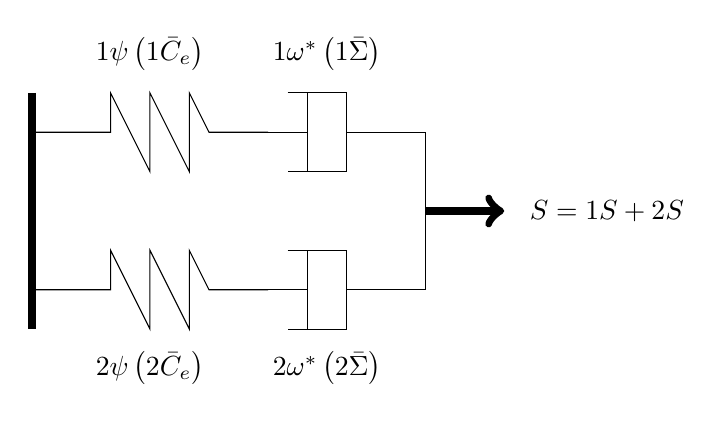
\begin{tikzpicture}
    % Spring 1
    \draw[-] (0,0) -- (1,0) -- (1,0.5) -- (1.5,-0.5) -- (1.5,0.5) -- (2,-0.5) -- (2,0.5) -- (2.25,0) -- (3,0);
    % dashpot 1
    \draw[-] (3,0) -- (3.5,0) -- (3.5,0.5) -- (3.5,-0.5);
    \draw[-] (3.25,0.5) -- (4,0.5) -- (4,-0.5) -- (3.25,-0.5);
    \draw[-] (4,0) -- (5,0);
    % Spring 2
    \draw[-] (0,0-2) -- (1,0-2) -- (1,0.5-2) -- (1.5,-0.5-2) -- (1.5,0.5-2) -- (2,-0.5-2) -- (2,0.5-2) -- (2.25,0-2) -- (3,0-2);
    % dashpot 2
    \draw[-] (3,0-2) -- (3.5,0-2) -- (3.5,0.5-2) -- (3.5,-0.5-2);
    \draw[-] (3.25,0.5-2) -- (4,0.5-2) -- (4,-0.5-2) -- (3.25,-0.5-2);
    \draw[-] (4,0-2) -- (5,0-2);
    % left boundary
    \draw[-,line width = 3pt] (0,0.5) -- (0,-2.5);
    % right boundary
    \draw[-] (5,0) -- (5,0-2);
    \draw[->,line width = 3pt] (5,-1) -- (6.0,-1);
    % description
    \node (psi1) [] at (1.5,1.0) {$\prescript{1}{}{}\psi\left(\prescript{1}{}{}\bar{\bm{C}}_e\right)$};
    \node (psi2) [] at (1.5,-3.0) {$\prescript{2}{}{}\psi\left(\prescript{2}{}{}\bar{\bm{C}}_e\right)$};
    \node (w1) [] at (3.75,1.0) {$\prescript{1}{}{}\omega^*\left(\prescript{1}{}{}\bar{\bm{\Sigma}}\right)$};
    \node (w2) [] at (3.75,-3.0) {$\prescript{2}{}{}\omega^*\left(\prescript{2}{}{}\bar{\bm{\Sigma}}\right)$};
    \node (S) [anchor=west] at (6.2,-1) {$\bm{S} = \prescript{1}{}{}\bm{S} + \prescript{2}{}{}\bm{S}$};
\end{tikzpicture}
    \caption{Rheological representation of the parallel connection of two generalized iCANNs. Each iCANN consists of an individual `spring', $\prescript{1}{}{}\psi$ or $\prescript{2}{}{}\psi$, and `dashpot', $\prescript{1}{}{}\omega^*$ or $\prescript{2}{}{}\omega^*$, element with individual states, $\prescript{1}{}{}\bm{U}_i$ and $\prescript{2}{}{}\bm{U}_i$, respectively. The entire Helmholtz free energy is $\psi = \prescript{1}{}{}\psi + \prescript{2}{}{}\psi$, while the overall dual potential is the sum of the individual potentials, i.e., $\omega^*=\prescript{1}{}{}\omega^* + \prescript{2}{}{}\omega^*$. For both individual iCANNs, the same right Cauchy-Green tensor, $\bm{C}$, serves as input. Consequently, the outputs are summed up to a single second Piola-Kirchhoff stress, $\bm{S}$.}
    \label{fig:rheo}
\end{figure}
%
%================================================
\subsection{Discovery of artificial data}
\label{sec:results_artificial}
%
In line with Shannon's information theory \cite{shannon1948}, `rich' data sets should enable us to discover a `unique' set of weights and biases; however, `rich' does not necessarily mean more data points.
Key features such as diverse data sets and higher information entropy prevent overfitting, while the performance during gradient optimization usually improves.
In terms of material science and computational discovery, we hypothesize that `rich' data sets featuring complex, relaxing, multiaxial, and cyclic load paths will help us to discover our weights in the network.
Thus, we prescribe the loading path shown in Figure~\ref{fig:loading} with $\Delta t = 0.05$ [min] to create a `rich' data set, which is utilized to obtain stress-time data in Sections~\ref{sec:results_artificial_1} and \ref{sec:results_artificial_2}.
To test our discovered weights and biases, we subject the network to uniaxial loading.
Here, we compute the remaining entries in Figure~\ref{fig:loading} (loading) according to the uniaxial stress constraint with $\Delta t = 0.06$ [min].
Noteworthy, the components of the deformation gradient may vary depending on the energy and potential employed.
%
\begin{figure}[h]
    \centering
    %\begin{tikzpicture}
\begin{axis} [
    grid = major,
    xlabel = {Time $t$ [min]},
    ylabel = {Stretch $F_{ij}$ [-]},
    width=0.45\textwidth,
    height=0.4\textwidth,
    /pgf/number format/1000 sep={},
    ymin = -0.5,
    ymax = 2.6,
    xmin = 0.0,
    xmax = 17.0,
    legend style={
        at={(0.5,1.05)}, % Position der Legende
        anchor=south % Verankerungspunkt
    },
    legend cell align = {left},
    legend columns=-1,
    title={Training}, % Title text
    title style={
        at={(0.95,0.90)}, % Position at the top-right
        anchor=north east, % Anchoring to the top-right
        font=\large, % Optional font size change
        fill=white, % Background color
        draw=black, % Border color (optional)
        rounded corners=3pt, % Optional rounded corners
        inner sep=6pt % Padding inside the box        
        }    
    ]
\addplot[rwth1, line width=2pt] table[x expr=\thisrowno{0},	y expr=\thisrowno{1}] {00_Original/graphs/prescribed_loading.txt};
\addplot[rwth8, line width=2pt] table[x expr=\thisrowno{0},	y expr=\thisrowno{2}] {00_Original/graphs/prescribed_loading.txt};
\addplot[rwth9, line width=2pt] table[x expr=\thisrowno{0},	y expr=\thisrowno{3}] {00_Original/graphs/prescribed_loading.txt};
\legend{$F_{11}(t)$,$F_{22}(t)$,$F_{12}(t)$}
\end{axis}
\end{tikzpicture}
\begin{tikzpicture}
\begin{axis} [
    grid = major,
    xlabel = {Time $t$ [min]},
    ylabel = {Stretch $F_{ij}$ [-]},
    width=0.45\textwidth,
    height=0.4\textwidth,
    /pgf/number format/1000 sep={},
    ymin = -0.5,
    ymax = 2.6,
    xmin = 0.0,
    xmax = 17.0,
    legend style={
        at={(0.5,1.05)}, % Position der Legende
        anchor=south % Verankerungspunkt
    },
    legend cell align = {left},
    legend columns=-1,
    title={Testing}, % Title text
    title style={
        at={(0.95,0.05)}, % Position at the top-right
        anchor=south east, % Anchoring to the top-right
        font=\large, % Optional font size change
        fill=white, % Background color
        draw=black, % Border color (optional)
        rounded corners=3pt, % Optional rounded corners
        inner sep=6pt % Padding inside the box        
        }    
    ]
\addplot[rwth4, line width=2pt] table[x expr=\thisrowno{0},	y expr=\thisrowno{1}] {00_Original/graphs/Model_v1_testing_F.txt};
\legend{$F_{11}(t)$}
\end{axis}
\end{tikzpicture}
    \includegraphics[]{figures/plot_prescribed_loading/Generalized-figure0.pdf}
    \includegraphics[]{figures/plot_prescribed_loading/Generalized-figure1.pdf}
    \caption{Left: Deformation gradient components used for creating a training data set. The third entry on the main diagonal, $F_{33}$, is set to one, while the remaining shear terms are zero. The training set includes multiaxial, cyclic, and relaxation behavior. Right: Prescribed stretch in the main stretch direction for uniaxial loading employed for testing. The remaining components of the deformation gradient are computed according to the constraint that the entries of $\bm{S}$ in the off-main diagonal direction are zero.}
    \label{fig:loading}
\end{figure}
%
%================================================
\subsubsection{Discovering a model for artificial data: Example 1}
\label{sec:results_artificial_1}
%
In this first example, we investigate the network's capabilities to discover the weights and biases of our proposed network in order to accurately describe the material behavior.
As alluded in the previous section, we create an artificial data set by subjecting a constitutive model to a complex loading path.
For the Helmholtz free energy and the dual potential, we use the following compressible Neo-Hookean model
%
\begin{align}
    \psi &= \frac{\mu}{2}\,\left(\tilde{I}_1^{\bar{\bm{C}}_e} - 3 \right) + \frac{\kappa}{4}\, \left( I_3^{\bar{\bm{C}}_e} - 1 - \mathrm{ln}\left(I_3^{\bar{\bm{C}}_e}\right)\right) + \frac{\mu}{2}\,\left(\tilde{I}_1^{\bm{C}} - 3 \right) + \frac{\kappa}{4}\, \left( I_3^{\bm{C}} - 1 - \mathrm{ln}\left(I_3^{\bm{C}}\right)\right) \label{eq:energy_artificial_1}\\
    \omega^* &= K_1\, \left(\mathrm{cosh}\left( \frac{J_3^{\bar{\bm{\Sigma}}}}{J_2^{\bar{\bm{\Sigma}}} + 1} \right) - 1 \right) \label{eq:potential_artificial_1}
\end{align}
%
with $\mu=1$ [MPa] and $\kappa=1$ [MPa], and $K_1=2$ [1/MPa].
From a rheological viewpoint, Equations~\eqref{eq:energy_artificial_1} and \eqref{eq:potential_artificial_1} describe a `spring' element connected in parallel to a Maxwell element.
Remarkably, the potential is not `analytically' included in the architecture of the network, but is otherwise arbitrary.
However, since neural networks serve as universal approximators, we want to explore the geneeralized iCANN's capabilities to discover this potential.
Additionally, the material parameters are chosen such that there is a high amount of energy dissipation present.
The components of the deformation gradient for testing are shown in Figure~\ref{fig:results_artificial_1_deformation}.
%
\begin{figure}[h]
    \centering
    %\begin{tikzpicture}
\begin{axis} [
    grid = major,
    xlabel = {Time $t$ [min]},
    ylabel = {Stretch $F_{22}(t)=F_{33}(t)$ [-]},
    width=0.45\textwidth,
    height=0.4\textwidth,
    /pgf/number format/1000 sep={},
    ymin = 0.5,
    ymax = 1.5,
    xmin = 0.0,
    xmax = 17.0,
    legend style={
        at={(0.5,1.05)}, % Position der Legende
        anchor=south % Verankerungspunkt
    },
    legend cell align = {left},
    legend columns=-1
    ]
\addplot[rwth5, line width=2pt] table[x expr=\thisrowno{0},	y expr=\thisrowno{2}] {00_Original/graphs/Model_v2_testing_F.txt};
\end{axis}
\end{tikzpicture}
    \includegraphics[]{figures/plot_Model_v2_F/Generalized-figure0.pdf}
    \caption{Components of the deformation gradient for uniaxial loading corresponding to the Helmholtz free energy~\eqref{eq:energy_artificial_1} and potential~\eqref{eq:potential_artificial_1} for the first example of artificial data.
    The loading path in the main direction is shown in Figure~\ref{fig:loading}. The remaining shear components of the deformation gradient are equal to zero.}
    \label{fig:results_artificial_1_deformation}
\end{figure}\newline
%

\textbf{Discovery.} The weights identified in this study are too numerous to enumerate in this manuscript\footnote{Comprehensive data on weights and biases is available online.}. 
However, key components of the weight vector, $\mathbf{w}_{\omega^*}$, are summarized in Table~\ref{tab:w_pot_artificial_1}, with the corresponding training loss illustrated in Figure~\ref{fig:loss_artificial_1}. 
Notably, during training, the iCANN autonomously identifies the components of the first Maxwell element, $\prescript{1}{}{}\mathbf{w}_{\omega^*}$, as a zero vector, while the second potential exhibits relative sparsity. 
This finding is significant as it aligns with the rheological model defined by Equations~\eqref{eq:energy_artificial_1}-\eqref{eq:potential_artificial_1}. 
If the weights associated with the final layer of the generalized potential are zero, it indicates that the iCANN effectively simplifies to a Constitutive Artificial Neural Network (CANN) focused solely on hyperelastic behavior.
Figure~\ref{fig:train_test_artificial_1} presents the training and testing results for the weights identified during training. 
We observe good agreement between the artificial data and the model's response in both training and testing phases.
The model is capable of adequately recovering the relaxation behavior, especially in the constant deformation states, e.g., from $t=2.5$ [min] up to $t=3.5$ [min].

Although the test results align well in the primary loading direction, \(\hat{S}_{11}\), an artificial stress increase is observed in the off-axis direction, \(\hat{S}_{22}\). 
This suggests that the discovered weights deviate from the exact solution. If they perfectly matched the artificial material model, \(\hat{S}_{22}\) should vanish under uniaxial tension (Figures~\ref{fig:loading} and \ref{fig:results_artificial_1_deformation}). 
Instead, the discovered weights induce a constrained deformation, analogous to the difference between Young's modulus and the longitudinal modulus in elasticity theory.
Whether this truly constitutes an `issue' is debatable. 
If the discovered network is used to simulate a boundary value problem, the strong form of equilibrium would enforce a uniaxial stress state, albeit with a different transverse elongation.
%
\begin{figure}[h]
    \centering
    %\begin{tikzpicture}
\begin{semilogyaxis} [grid = major,
    			xlabel = {epochs},
    			ylabel = {Training loss $L$},
    			width=0.45\textwidth,
    			height=0.4\textwidth,
    			/pgf/number format/1000 sep={},		
		]
    		 \addplot[rwth1, line width=2pt, smooth] table[x expr=\coordindex+1, y index=0] {00_Original/graphs/Model_v2_losses.txt};
\end{semilogyaxis}
\end{tikzpicture}
    \includegraphics[]{figures/plot_Model_v2_loss/Generalized-figure0.pdf}
    \caption{Loss during training of the generalized iCANN for the first example of artificially generated data. The loss is plotted on a logarithmic scale. For training, $3000$ epochs were used.}
    \label{fig:loss_artificial_1}
\end{figure}
%
\begin{figure}[h]
    \centering
    %\begin{tikzpicture}
\begin{axis} [
    grid = major,
    xlabel = {Time $t$ [min]},
    ylabel = {Stress $S_{ij}$ [MPa]},
    width=0.9\textwidth,
    height=0.4\textwidth,
    /pgf/number format/1000 sep={},
    ymin = -5.0,
    ymax = 3.0,
    xmin = 0.0,
    xmax = 17.0,
    legend style={
        at={(0.5,1.05)}, % Position der Legende
        anchor=south % Verankerungspunkt
    },
    legend cell align = {left},
    legend columns=-1,
    title={Training}, % Title text
    title style={
        at={(0.95,0.05)}, % Position at the top-right
        anchor=south east, % Anchoring to the top-right
        font=\large, % Optional font size change
        fill=white, % Background color
        draw=black, % Border color (optional)
        rounded corners=3pt, % Optional rounded corners
        inner sep=6pt % Padding inside the box        
        }
    ]
\addplot[red, smooth,
        line width=2pt] table[x expr=\thisrowno{0},	y expr=\thisrowno{14}] {00_Original/graphs/Model_v2_training_time.txt};
\addplot[blue, 
        line width=2pt] table[x expr=\thisrowno{0},	y expr=\thisrowno{15}] {00_Original/graphs/Model_v2_training_time.txt};
\addplot[lightblue, 
        line width=2pt] table[x expr=\thisrowno{0},	y expr=\thisrowno{17}] {00_Original/graphs/Model_v2_training_time.txt};
\addplot[cyan, 
        mark=o,
        mark size=1.0pt,
        only marks,
        line width=0pt] table[x expr=\thisrowno{0},	y expr=\thisrowno{8}] {00_Original/graphs/Model_v2_training_time.txt};
\addplot[yellow, 
        mark=o,
        mark size=1.0pt,
        only marks,
        line width=0pt] table[x expr=\thisrowno{0},	y expr=\thisrowno{9}] {00_Original/graphs/Model_v2_training_time.txt};
\addplot[orange, 
        mark=o,
        mark size=1.0pt,
        only marks,
        line width=0pt] table[x expr=\thisrowno{0},	y expr=\thisrowno{11}] {00_Original/graphs/Model_v2_training_time.txt};        
\legend{$S_{11}(t)$,$S_{22}(t)$,$S_{12}(t)$,$\hat{S}_{11}(t)$,$\hat{S}_{22}(t)$,$\hat{S}_{12}(t)$}
\end{axis}
\end{tikzpicture}

\begin{tikzpicture}
\begin{axis} [
    grid = major,
    xlabel = {Time $t$ [min]},
    ylabel = {Stress $S_{ij}$ [MPa]},
    width=0.9\textwidth,
    height=0.4\textwidth,
    /pgf/number format/1000 sep={},
    ymin = -18.5,
    ymax = 2.0,
    xmin = 0.0,
    xmax = 17.0,
    legend style={
        at={(0.5,1.05)}, % Position der Legende
        anchor=south % Verankerungspunkt
    },
    legend cell align = {left},
    legend columns=-1,
    title={Testing}, % Title text
    title style={
        at={(0.95,0.05)}, % Position at the top-right
        anchor=south east, % Anchoring to the top-right
        font=\large, % Optional font size change
        fill=white, % Background color
        draw=black, % Border color (optional)
        rounded corners=3pt, % Optional rounded corners
        inner sep=6pt % Padding inside the box        
        }
    ]
\addplot[red, smooth,
        line width=2pt] table[x expr=\thisrowno{0},	y expr=\thisrowno{14}] {00_Original/graphs/Model_v2_testing_time.txt};
\addplot[blue, 
        line width=2pt] table[x expr=\thisrowno{0},	y expr=\thisrowno{15}] {00_Original/graphs/Model_v2_testing_time.txt};
\addplot[lightblue, 
        line width=2pt] table[x expr=\thisrowno{0},	y expr=\thisrowno{17}] {00_Original/graphs/Model_v2_testing_time.txt};
\addplot[cyan, 
        mark=o,
        mark size=1.0pt,
        only marks,
        line width=0pt] table[x expr=\thisrowno{0},	y expr=\thisrowno{8}] {00_Original/graphs/Model_v2_testing_time.txt};
\addplot[yellow, 
        mark=o,
        mark size=1.0pt,
        only marks,
        line width=0pt] table[x expr=\thisrowno{0},	y expr=\thisrowno{9}] {00_Original/graphs/Model_v2_testing_time.txt};
\addplot[orange, 
        mark=o,
        mark size=1.0pt,
        only marks,
        line width=0pt] table[x expr=\thisrowno{0},	y expr=\thisrowno{11}] {00_Original/graphs/Model_v2_testing_time.txt};
%\addplot[gray, thick] coordinates {(0,-0.5) (16,-0.5) (16,0.5) (0,0.5) (0,0.5)};
\end{axis}
% Zoom window
\begin{axis}[
        at={(40.0,100.0)}, % Position of the zoom window (relative)
        anchor=south west, % Anchor point for positioning
        width=0.4\textwidth, 
        height=0.2\textwidth,
        xmin=0.0, xmax=17,
        ymin=-0.5, ymax=0.5,
        xtick=\empty,
        grid = major,
        axis background/.style={fill=white}
    ]
    \addplot[blue, 
        line width=2pt] table[x expr=\thisrowno{0},	y expr=\thisrowno{15}] {00_Original/graphs/Model_v2_testing_time.txt};
    \addplot[yellow, 
        mark=o,
        mark size=1.0pt,
        only marks,
        line width=0pt] table[x expr=\thisrowno{0},	y expr=\thisrowno{9}] {00_Original/graphs/Model_v2_testing_time.txt};        
    \end{axis}
\end{tikzpicture}
    \includegraphics[]{figures/plot_Model_v2/Generalized-figure0.pdf}

    \includegraphics[]{figures/plot_Model_v2/Generalized-figure1.pdf}    
    \caption{Discovered model for the first example of artificially generated data. The predicted stress components, $S_{ij}$, are plotted against the artificially generated data, $\hat{S}_{ij}$. Above: Training results for the discovered weights of multiaxial loading. Below: Testing results for uniaxial tension. The zoomed window shows stresses $S_{22}$ and $\hat{S}_{22}$ over the entire load path up to $t=16$ [min].}
    \label{fig:train_test_artificial_1}
\end{figure}\newline
%

\textbf{Implicit discovery.} Up to now, we have determined the network's weights and biases using an explicit exponential integrator scheme. 
However, implicit time integration schemes are more commonly employed in computational mechanics due to their superior stability and robustness. 

To investigate this, we trained the implicit version of the generalized iCANN using the same data set. 
The results, shown in Figure~\ref{fig:implicit_artificial_1}, reveal that both weight vectors, \(\prescript{1}{}{}\mathbf{w}_{\omega^*} = \prescript{2}{}{}\mathbf{w}_{\omega^*} = \mathbf{0}\), reduce to the zero vector. 
This implies that the iCANN collapses entirely into a CANN, rendering it incapable of representing inelastic material behavior. 
Consequently, we observe a strong discrepancy in the training results.

To further analyze this behavior, we evaluate the implicit network using the weights obtained from the explicit scheme (see Figure~\ref{fig:train_test_artificial_1}). 
Up to \(t = 7.35\) [min], the results align well with the training data. 
However, beyond this point, the local Broyden iteration fails to converge. 
This suggests that greater attention must be given to developing a stable and robust iterative solving technique, though this is beyond the scope of this study. 
Nevertheless, Section~\ref{sec:discussion} provides a more detailed discussion on the implementation of the implicit integration scheme.
%
\begin{table}[t]
    \centering
    %\resizebox{\textwidth}{!}{
        \begin{tabular}{l | l l l l l l l l}
                &   1   &   2   &   3   &   4   &   5   &   6   &   7   &   8 \\
            \hline
            $\prescript{1}{}{}\mathbf{w}_{\omega^*}$ & $0$ & $0$ & $0$ & $0$ & $0$ & $0$ & $0$ & $0$ \\
            $\prescript{2}{}{}\mathbf{w}_{\omega^*}$ & $0$ & $0.2103749$ & $0$ & $0$ & $0$ & $0$ & $0$ & $0$
        \end{tabular}
    %}
    \caption{First example of artificially generated data. Listed are the components of the weight vector, $\mathbf{w}_{\omega^*}$, for the generalized iCANN shown in Figure~\ref{fig:rheo}. The first four weights correspond to the maximum activation function, while the latter four correspond to the exponential activation.}
    \label{tab:w_pot_artificial_1}
\end{table}
%
\begin{figure}[h]
    \centering
    %\input{graphs/plot_Model_v2_comp_integration}
    \includegraphics[]{figures/plot_Model_v2_comp_integration/Generalized-figure0.pdf}

    \includegraphics[]{figures/plot_Model_v2_comp_integration/Generalized-figure1.pdf}
    \caption{\textbf{Implicit discovery.} Above: Discovered model for the first example of artificially generated data with an implicit time integration scheme. The network's weights for the generalized dual potential, $\prescript{1}{}{}\mathbf{w}_{\omega^*}$ and $\prescript{2}{}{}\mathbf{w}_{\omega^*}$, turn out to be the zero vector. Thus, the network behaves as a purely elastic network (CANN). Below: Predicted stresses for the generalized iCANN with implicit time integration but employing the discovered weights and biases of the explicit architecture (cf. Figure~\ref{fig:train_test_artificial_1}). The local iteration aborts after $t=7.35$ [min].}
    \label{fig:implicit_artificial_1}
\end{figure}
%
%
\FloatBarrier
%================================================
\subsubsection{Discovering a model for artificial data: Example 2}
\label{sec:results_artificial_2}
%
We proceed by evaluating the performance of the generalized iCANN using a different constitutive model.
For the Helmholtz free energy, we stick to the very same energy~\eqref{eq:energy_artificial_1} as in the first example, however, we exchange the potential~\eqref{eq:potential_artificial_1} by a quadratic form, i.e.,
%
\begin{equation}
    \omega^* = K_1\, \left(2\,J_2^{\bar{\bm{\Sigma}}}\right) + K_2\, \left(I_2^{\bar{\bm{\Sigma}}}\right)^2
\label{eq:potential_artificial_2}
\end{equation}
%
with $\mu=25$ [MPa], $\kappa=50$ [MPa], $K_1=4 \cdot 10^{-5}$ [1/MPa], and $K_2=7.2 \cdot 10^{-4}$ [1/MPa].
The shear modulus, $\mu$, as well as the bulk modulus, $\kappa$, are also used to determine the Helmholtz free energy~\eqref{eq:energy_artificial_1}.
As in the first example, the constitutive model represents a Maxwell and a `spring' element connected in parallel.
However, contrary to the first example, the choice of material parameters yields a small amount of energy dissipation compared to the elastic response of the `spring'.
To create artificial data sets for training and testing, we subject the constitutive model (Equations~\eqref{eq:energy_artificial_1} and \eqref{eq:potential_artificial_2}) to the loadings described in Figure~\ref{fig:loading}.
The remaining components of the deformation gradient to achieve a state of uniaxial tension are shown in Figure~\ref{fig:results_artificial_2_deformation}.\newline

\textbf{Discovery.} For the chosen material parameters, the training stresses exceed $100$ [MPa], causing the iteration to abort. 
To address this, we normalize the artificial data by the absolute maximum stress value, \( S^{\text{max}} = 125.1517 \) [MPa], as is common in neural network training.

Figure~\ref{fig:train_full_artificial_2} presents the training results. 
As in the first example, the entire load path up to \( t = 17 \) [min], consisting of 341 data points, is used for training. 
Once again, the iCANN autonomously identifies that the weights of one Maxwell element vanish while the other retain nonzero values. 
However, the predicted stresses exhibit poor agreement with the artificial data, particularly in capturing the relaxation behavior.

This discrepancy raises the question of its origin. 
Given that the same complex loading path is used, the issue is unlikely due to insufficient data richness. 
A potential bottleneck, particularly for inelastic materials, may be the initialization of the weights.\newline 

\textbf{Staggered discovery.} To investigate our assumption regarding initialization, we vary the batch size used for training, i.e., we do not utilize the full data set at once. 
Instead, we start with a smaller subset of the 341 data points. 

Although varying the batch size is a common practice in neural network training and can be applied to CANNs, inelastic materials require special treatment. 
Due to the strong sequential dependency imposed by the time integration scheme, randomly selecting data points is not feasible. 
Instead, each training batch must consist of a continuous sequence of data points.
Furthermore, even when using sequential subsets, the initial values of the internal states remain unknown. 
Consequently, every batch must begin at the very start of the entire load path to ensure consistency in training.

In this contribution, we introduce a staggered discovery scheme, where training begins with a small subset of data points. 
The subset is then incrementally expanded while initializing each new training phase with the discovered weights from the previous step. 
This process is repeated until the entire load path is used for training.
For the current study, we employ three subsets: 70 data points, 170 data points, and 240 data points. 
The training losses for all sessions are plotted in Figure~\ref{fig:loss_artificial_2}, while the discovered weights of the last layer of the generalized potential are listed in Table~\ref{tab:w_pot_artificial_2}. 
Figure~\ref{fig:train_test_artificial_2} presents both the training and testing results.

It is noteworthy that the staggered discovery scheme yields better agreement with the artificial data, particularly in capturing the relaxation behavior, compared to the initial approach (cf. Figure~\ref{fig:train_full_artificial_2}). 
Once again, the iCANN autonomously identifies the visco-elastic nature of the data, as one iCANN reduces to a CANN network.
Although the potential is explicitly incorporated into the proposed network architecture, some discrepancies remain, indicating that the network has not yet discovered the optimal solution. 
Interestingly, despite the inclusion of the quadratic potential, the discovered weights in Table~\ref{tab:w_pot_artificial_2} reveal that only the weights associated with the exponential activation function are nonzero.

During testing, the predicted responses align well with the artificial data for most of the loading path, except at the second peak stress. 
This discrepancy may be attributed to the exponential activation function, which grows rapidly with increasing stress. 
Consequently, its incorrect influence may manifest only at high stress levels and was likely negligible during training.
As in the first example, an artificial increase in off-axis stresses is observed throughout the testing session. 
The underlying cause of this phenomenon is similar to the explanation provided in Section~\ref{sec:results_artificial_2}.

In this study, we did not adjust hyperparameters such as the number of layers, neurons, or activation functions, nor did we refine weight initialization. 
These factors may influence our findings (see Section~\ref{sec:discussion} for further discussion).\newline

\textbf{Discover noisy data.} So far, we have considered `clean' data generated deterministically from the constitutive model. 
However, real measurement data often contain noise. 
To evaluate the stability of our chosen regularization technique against overfitting, we introduce white Gaussian noise into our training data. 
We apply the staggered discovery scheme once again. 
The training results are presented in Figure~\ref{fig:train_test_artificial_noisy_2}, while losses are plotted in Figure~\ref{fig:loss_artificial_2}. 
Table~\ref{tab:w_pot_artificial_2} lists the weights discovered in the last layer of the generalized iCANN. 
The discovered model aligns well with the noisy data, showing no signs of overfitting; additionally, its qualitative response resembles that without noise. 
Notably, the same neuron is activated. 
However, it can be assumed that stress predictions may diverge from artificial data for higher stress peaks due to greater variability in inelastic stretch evolution.
%
\begin{table}[h]
    \centering
    %\resizebox{\textwidth}{!}{
        \begin{tabular}{l l | l l l l l l l l}
                &    &   1   &   2   &   3   &   4   &   5   &   6   &   7   &   8 \\
            \hline
            \multirow{2}{*}{Clean}  & $\prescript{1}{}{}\mathbf{w}_{\omega^*}$ & $0$ & $0$ & $0$ & $0$ & $0.00452437$ & $0$ & $0$ & $0$ \\
                                    & $\prescript{2}{}{}\mathbf{w}_{\omega^*}$ & $0$ & $0$ & $0$ & $0$ & $0$ & $0$ & $0$ & $0$ \\
            \hline
            \multirow{2}{*}{Noisy}  & $\prescript{1}{}{}\mathbf{w}_{\omega^*}$ & $0$ & $0$ & $0$ & $0$ & $0.086715$ & $0$ & $0$ & $0$ \\
                                    & $\prescript{2}{}{}\mathbf{w}_{\omega^*}$ & $0$ & $0$ & $0$ & $0$ & $0$ & $0$ & $0$ & $0$                                    
        \end{tabular}
    %}
    \caption{Second example of artificially generated data. Listed are the components of the weight vector, $\mathbf{w}_{\omega^*}$, for the generalized iCANN shown in Figure~\ref{fig:rheo}. The first four weights correspond to the maximum activation function, while the latter four correspond to the exponential activation. Both the weights for the clean data set (see Figure~\ref{fig:train_test_artificial_2}) and the noisy data set (see Figure~\ref{fig:train_test_artificial_noisy_2}) are shown.}
    \label{tab:w_pot_artificial_2}
\end{table}
%
\begin{figure}[h]
    \centering
    %\input{graphs/plot_Model_v1_F}
    \includegraphics[]{figures/plot_Model_v1_F/Generalized-figure0.pdf}
    \caption{Components of the deformation gradient for uniaxial loading corresponding to the Helmholtz free energy~\eqref{eq:energy_artificial_1} and potential~\eqref{eq:potential_artificial_2} for the second example of artificial data.
    The loading path in the main direction is shown in Figure~\ref{fig:loading}. The remaining shear components of the deformation gradient are equal to zero.}
    \label{fig:results_artificial_2_deformation}
\end{figure}
%
\begin{figure}[h]
    \centering
    %\input{graphs/plot_Model_v1}
    \includegraphics[]{figures/plot_Model_v1/Generalized-figure0.pdf}
    \caption{\textbf{Full data discovery.} Discovered model for the second example of artificially generated data. The predicted stress components, \( S_{ij} \), are plotted against the normalized artificially generated data, \( \hat{S}_{ij} \). The data are normalized by \( S^{\text{max}} = 125.1517 \) [MPa]. The entire load path, consisting of 341 data points, is used simultaneously for training.}
    \label{fig:train_full_artificial_2}
\end{figure}
%
\begin{figure}[h]
    \centering
    %\begin{tikzpicture}
\begin{semilogyaxis} [grid = major,
    			xlabel = {epochs},
    			ylabel = {Training loss $L$},
    			width=0.45\textwidth,
    			height=0.4\textwidth,
    			/pgf/number format/1000 sep={},
    legend pos = north east,
    legend cell align={left},
    title = {Clean data},
    title style={
        fill=white, % Background color
        draw=black, % Border color (optional)
        rounded corners=3pt, % Optional rounded corners
        inner sep=6pt % Padding inside the box        
        }     
		]
    \addplot[rwth1, line width=2pt, smooth] table[x expr=\coordindex+1, y index=0] {00_Original/graphs/Model_v1_norm0_losses.txt};
    \addplot[rwth5, line width=2pt, smooth] table[x expr=\coordindex+1, y index=0] {00_Original/graphs/Model_v1_norm1_losses.txt};
    \addplot[rwth6, line width=2pt, smooth] table[x expr=\coordindex+1, y index=0] {00_Original/graphs/Model_v1_norm2_losses.txt};
    \addplot[rwth8, line width=2pt, smooth] table[x expr=\coordindex+1, y index=0] {00_Original/graphs/Model_v1_norm3_losses.txt};
\legend{$n_{\text{data}}=70$,$n_{\text{data}}=170$,$n_{\text{data}}=240$,$n_{\text{data}}=341$}
\end{semilogyaxis}
\end{tikzpicture}
%
\begin{tikzpicture}
\begin{semilogyaxis} [grid = major,
    			xlabel = {epochs},
    			ylabel = {Training loss $L$},
    			width=0.45\textwidth,
    			height=0.4\textwidth,
    			/pgf/number format/1000 sep={},
    legend pos = north east,
    legend cell align={left},
    title = {Noisy data},
    title style={
        fill=white, % Background color
        draw=black, % Border color (optional)
        rounded corners=3pt, % Optional rounded corners
        inner sep=6pt % Padding inside the box        
        }       
		]
    \addplot[rwth1, line width=2pt, smooth] table[x expr=\coordindex+1, y index=0] {00_Original/graphs/Model_v1_norm_noise0_losses.txt};
    \addplot[rwth5, line width=2pt, smooth] table[x expr=\coordindex+1, y index=0] {00_Original/graphs/Model_v1_norm_noise1_losses.txt};
    \addplot[rwth6, line width=2pt, smooth] table[x expr=\coordindex+1, y index=0] {00_Original/graphs/Model_v1_norm_noise2_losses.txt};
    \addplot[rwth8, line width=2pt, smooth] table[x expr=\coordindex+1, y index=0] {00_Original/graphs/Model_v1_norm_noise3_losses.txt};
\legend{$n_{\text{data}}=70$,$n_{\text{data}}=170$,$n_{\text{data}}=240$,$n_{\text{data}}=341$}
\end{semilogyaxis}
\end{tikzpicture}
    \includegraphics[]{figures/plot_Model_v1_staggered_loss/Generalized-figure0.pdf}
    \includegraphics[]{figures/plot_Model_v1_staggered_loss/Generalized-figure1.pdf}
    \caption{Losses during training of the generalized iCANN for the second example of artificially generated data. The losses are plotted on a logarithmic scale. For training, $3000$ epochs were used. A staggered discovery scheme is employed, i.e., the data points used for training are gradually increased. Left: Losses for the `clean' data set, see Figure~\ref{fig:train_test_artificial_2}. Right: Losses for the `noisy' data set, see Figure~\ref{fig:train_test_artificial_noisy_2}.}
    \label{fig:loss_artificial_2}
\end{figure}
%
\begin{figure}[h]
    \centering
    %\begin{tikzpicture}
\begin{axis} [
    grid = major,
    xlabel = {Time $t$ [min]},
    ylabel = {Normalized stress $S_{ij}$ [-]},
    width=0.9\textwidth,
    height=0.4\textwidth,
    /pgf/number format/1000 sep={},
    ymin = -1.2,
    ymax = 1.0,
    xmin = 0.0,
    xmax = 17.0,
    legend style={
        at={(0.5,1.05)}, % Position der Legende
        anchor=south % Verankerungspunkt
    },
    legend cell align = {left},
    legend columns=-1,
    title={Training}, % Title text
    title style={
        at={(0.95,0.05)}, % Position at the top-right
        anchor=south east, % Anchoring to the top-right
        font=\large, % Optional font size change
        fill=white, % Background color
        draw=black, % Border color (optional)
        rounded corners=3pt, % Optional rounded corners
        inner sep=6pt % Padding inside the box        
        }    
    ]
\addplot[red, smooth,
        line width=2pt] table[x expr=\thisrowno{0},	y expr=\thisrowno{14}] {00_Original/graphs/Model_v1_norm_staggered_training_time.txt};
\addplot[blue, 
        line width=2pt] table[x expr=\thisrowno{0},	y expr=\thisrowno{15}] {00_Original/graphs/Model_v1_norm_staggered_training_time.txt};
\addplot[lightblue, 
        line width=2pt] table[x expr=\thisrowno{0},	y expr=\thisrowno{17}] {00_Original/graphs/Model_v1_norm_staggered_training_time.txt};
\addplot[cyan, 
        mark=o,
        mark size=1.0pt,
        only marks,
        line width=0pt] table[x expr=\thisrowno{0},	y expr=\thisrowno{8}] {00_Original/graphs/Model_v1_norm_staggered_training_time.txt};
\addplot[yellow, 
        mark=o,
        mark size=1.0pt,
        only marks,
        line width=0pt] table[x expr=\thisrowno{0},	y expr=\thisrowno{9}] {00_Original/graphs/Model_v1_norm_staggered_training_time.txt};
\addplot[orange, 
        mark=o,
        mark size=1.0pt,
        only marks,
        line width=0pt] table[x expr=\thisrowno{0},	y expr=\thisrowno{11}] {00_Original/graphs/Model_v1_norm_staggered_training_time.txt};        
\legend{$S_{11}(t)$,$S_{22}(t)$,$S_{12}(t)$,$\hat{S}_{11}(t)$,$\hat{S}_{22}(t)$,$\hat{S}_{12}(t)$}
\end{axis}
\end{tikzpicture}

\begin{tikzpicture}
\begin{axis} [
    grid = major,
    xlabel = {Time $t$ [min]},
    ylabel = {Stress $S_{ij}$ [MPa]},
    width=0.9\textwidth,
    height=0.4\textwidth,
    /pgf/number format/1000 sep={},
    ymin = -1000.0,
    ymax = 100.0,
    xmin = 0.0,
    xmax = 17.0,
    legend style={
        at={(0.5,1.05)}, % Position der Legende
        anchor=south % Verankerungspunkt
    },
    legend cell align = {left},
    legend columns=-1,
    title={Testing}, % Title text
    title style={
        at={(0.95,0.05)}, % Position at the top-right
        anchor=south east, % Anchoring to the top-right
        font=\large, % Optional font size change
        fill=white, % Background color
        draw=black, % Border color (optional)
        rounded corners=3pt, % Optional rounded corners
        inner sep=6pt % Padding inside the box        
        }    
    ]
\addplot[red, smooth,
        line width=2pt] table[x expr=\thisrowno{0},	y expr=\thisrowno{14}*125.1517] {00_Original/graphs/Model_v1_norm_staggered_testing_time.txt};
\addplot[blue, 
        line width=2pt] table[x expr=\thisrowno{0},	y expr=\thisrowno{15}*125.1517] {00_Original/graphs/Model_v1_norm_staggered_testing_time.txt};
\addplot[lightblue, 
        line width=2pt] table[x expr=\thisrowno{0},	y expr=\thisrowno{17}*125.1517] {00_Original/graphs/Model_v1_norm_staggered_testing_time.txt};
\addplot[cyan, 
        mark=o,
        mark size=1.0pt,
        only marks,
        line width=0pt] table[x expr=\thisrowno{0},	y expr=\thisrowno{8}] {00_Original/graphs/Model_v1_norm_staggered_testing_time.txt};
\addplot[yellow, 
        mark=o,
        mark size=1.0pt,
        only marks,
        line width=0pt] table[x expr=\thisrowno{0},	y expr=\thisrowno{9}] {00_Original/graphs/Model_v1_norm_staggered_testing_time.txt};
\addplot[orange, 
        mark=o,
        mark size=1.0pt,
        only marks,
        line width=0pt] table[x expr=\thisrowno{0},	y expr=\thisrowno{11}] {00_Original/graphs/Model_v1_norm_staggered_testing_time.txt};
\end{axis}
\end{tikzpicture}
    \includegraphics[]{figures/plot_Model_v1_staggered/Generalized-figure0.pdf}

    \includegraphics[]{figures/plot_Model_v1_staggered/Generalized-figure1.pdf}
    \caption{\textbf{Staggered discovery with clean data.} Discovered model for the second example of artificially generated data. The predicted stress components, $S_{ij}$, are plotted against the artificially generated data, $\hat{S}_{ij}$. Above: Training results for the discovered weights of multiaxial loading. The stresses are normalized by \( S^{\text{max}} = 125.1517 \) [MPa]. Below: Testing results for uniaxial tension. The stresses are not normalized.}
    \label{fig:train_test_artificial_2}
\end{figure}
%
\begin{figure}[h]
    \centering
    %\input{graphs/plot_Model_v1_noise_staggered}
    \includegraphics[]{figures/plot_Model_v1_noise_staggered/Generalized-figure0.pdf}
    \caption{\textbf{Staggered discovery with noisy data.} Discovered model for the second example of artificially generated data. The predicted stress components, $S_{ij}$, are plotted against the artificially generated data, $\hat{S}_{ij}$. White Gaussian noise is added to the data shown in Figure~\ref{fig:train_test_artificial_2}.}
    \label{fig:train_test_artificial_noisy_2}
\end{figure}
%
%
\FloatBarrier
%================================================
\subsection{Discovering a model for the experimental data of VHB 4910 polymer}
\label{sec:Hossain2012}
%
In this final example, we investigate the generalized iCANN's ability to model experimentally measured data. 
We utilize experimental data from very-high-bond (VHB) 4910 polymer published by \citet{hossain2012}, which has previously been used to assess the original iCANN formulation \cite{holthusen2024} and has been compared with other constitutive neural network approaches \cite{AbdolaziziLinkaEtAl2023} as well as a classical constitutive model \cite{hossain2012}. 
In these comparisons, the iCANN demonstrated strong performance and effectively predicted outside the training regime. 
Thus, this example also facilitates a comparison between our newly proposed iCANN and existing methodologies.

The polymer is subjected to constant uniaxial loading followed by uniaxial unloading at three distinct but constant rates. 
Several experiments were conducted with varying maximum stretch levels, specifically $ C_{11}^{\text{max}} \in \{2.25, 4.0, 6.25, 9.0\} $ [-]. 
Notably, no experimental data is provided for a deformation rate of $ 0.03 $ [1/s] at the maximum stretch level applied. 
In contrast to our previous examples, the time increment in this case is not constant, and we normalize the stress data to its maximum value of $ S^{\text{max}} = 27.988124 $ [kPa].

The data is one-dimensional; thus, no information on transverse elongation is provided. 
This results in an undetermined problem, leading us to assume incompressibility in line with prior studies \cite{holthusen2024,holthusen2024PAMM,AbdolaziziLinkaEtAl2023}. 
For details on implementing incompressibility, interested readers are referred to the original iCANN work \cite{holthusen2024}.\newline

\textbf{Discovery: Training A.} We begin with the same training setup as in \cite{holthusen2024}, utilizing only the data for $ C_{11}^{\text{max}} = 9.0 $ [-] for training. 
The corresponding loss during training is depicted in Figure~\ref{fig:Hossain2012_losses}, while the weights of the last layer of the potential are presented in Table~\ref{tab:w_pot_Hossain2012}. 
Notably, we do not use the deformation rate of $ 0.03 $ [1/s] for training, leaving this rate unseen by the network. 
Furthermore, for the experimental data, the iCANN autonomously discovers visco-elasticity by reducing one iCANN to a CANN architecture, resulting in zero weights.

In contrast to identifying material parameters for classical constitutive models \cite{hossain2012}, we omit multi-step relaxation data from the training. 
Our training and testing results are shown in Figure~\ref{fig:Hossain2012_training_A}. 
While there is good agreement during training, the model does not perform well on testing data; few predictions match well, e.g., for $ C_{11}^{\text{max}} = 4.0 $ [-] with a constant deformation rate of $0.05$, while most do not.

A plausible explanation has been provided by \citet{AbdolaziziLinkaEtAl2023}: 
The experimental data exhibit inconsistencies; for identical loading rates but different maximum stretch levels, the loading paths should align, which is not observed (see \cite{holthusen2024}). 
Consequently, a neural network based on constitutive equations -- including our generalized iCANN -- struggles to predict such stress curves.

Despite our new proposed iCANN performing well during training, it is less accurate compared to previous works \cite{hossain2012,AbdolaziziLinkaEtAl2023} and particularly when compared to the original iCANN \cite{holthusen2024}. 
This may seem surprising at first, as the original architecture is included within the new one.

However, while the original architecture consists of only nine weights per Maxwell element for the feed-forward network of the potential, our new architecture employs 316 weights (see Section~\ref{sec:architecture_potential}). 
Thus, it is not surprising that one-dimensional data may lack sufficient complexity to accurately determine all network weights. 
Considering Shannon's information theory \cite{shannon1948} alongside our results from artificially generated data sets with richer information could provide insight into this issue (see also Section~\ref{sec:discussion}).

Lastly, we note that four Maxwell elements were used in the original iCANN architecture to adequately recover stress responses and that it was initialized with a `spring' (CANN) element.
In contrast, our newly proposed architecture autonomously reduces complexity and requires only a single Maxwell element within the generalized iCANN framework to accurately recover stress responses during training.\newline

\textbf{Discovery: Training B.} The results from Training A indicate the need for additional data to enhance model discovery. 
Therefore, we incorporate not only the data for $ C_{11}^{\text{max}} = 9.0 $ [-] but also that for $ C_{11}^{\text{max}} = 4.0 $ [-], including all three deformation rates in the training process.

The loss is illustrated in Figure~\ref{fig:Hossain2012_losses}, and the discovered weights are detailed in Table~\ref{tab:w_pot_Hossain2012}. 
Once again, the iCANN autonomously identifies the underlying mechanisms of visco-elasticity by reducing one iCANN to a CANN. 
Our training and testing results are presented in Figure~\ref{fig:Hossain2012_training_B}.

Although performance improves within the training regime due to this richer dataset compared to Figure~\ref{fig:Hossain2012_training_A}, predictions outside this regime remain poor relative to earlier studies. 
While qualitative stress responses may be recovered, quantitative curves do not align well. 
The iCANN continues to struggle with insufficiently `rich' data for accurately determining weights and biases relevant to the material under investigation.

As previously noted, stresses should ideally match for identical deformation rates. 
Consequently, the additional data from $ C_{11}^{\text{max}} = 4.0 $ [-] primarily introduces previously unseen deformation rates and unloading curves. 
Whether this sufficiently enhances the richness of one-dimensional data for discovering numerous weights remains questionable (see also Section~\ref{sec:discussion}).
%
\begin{table}[t]
    \centering
    %\resizebox{\textwidth}{!}{
        \begin{tabular}{l l | l l l l l l l l}
                &    &   1   &   2   &   3   &   4   &   5   &   6   &   7   &   8 \\
            \hline
            \multirow{2}{*}{Training A}  & $\prescript{1}{}{}\mathbf{w}_{\omega^*}$ & $0$ & $0$ & $0$ & $0$ & $0.19749504$ & $0$ & $0$ & $0$ \\
                                    & $\prescript{2}{}{}\mathbf{w}_{\omega^*}$ & $0$ & $0$ & $0$ & $0$ & $0$ & $0$ & $0$ & $0$ \\
            \hline
            \multirow{2}{*}{Training B}  & $\prescript{1}{}{}\mathbf{w}_{\omega^*}$ & $0$ & $0$ & $0$ & $0$ & $0.09977169$ & $0$ & $0$ & $0$ \\
                                    & $\prescript{2}{}{}\mathbf{w}_{\omega^*}$ & $0$ & $0$ & $0$ & $0$ & $0$ & $0$ & $0$ & $0$                                    
        \end{tabular}
    %}
    \caption{Experimental data of VHB 4910 polymer \cite{hossain2012}. Listed are the components of the weight vector, $\mathbf{w}_{\omega^*}$, for the generalized iCANN shown in Figure~\ref{fig:rheo}. The first four weights correspond to the maximum activation function, while the latter four correspond to the exponential activation. Both the weights for the training session A (see Figure~\ref{fig:Hossain2012_training_A}) and training session B (see Figure~\ref{fig:Hossain2012_training_B}) are shown.}
    \label{tab:w_pot_Hossain2012}
\end{table}
%
\begin{figure}[h]
    \centering
    \begin{tikzpicture}
\begin{semilogyaxis} [grid = major,
    			xlabel = {epochs},
    			ylabel = {Training loss $L$},
    			width=0.45\textwidth,
    			height=0.4\textwidth,
    			/pgf/number format/1000 sep={},
    legend pos = north east,
    legend cell align={left}   
		]
    \addplot[rwth1, line width=2pt, smooth] table[x expr=\coordindex+1, y index=0] {graphs/Hossain2012_Fig42_losses.txt};
    \addplot[rwth5, line width=2pt, smooth] table[x expr=\coordindex+1, y index=0] {graphs/Hossain2012_Fig42_Fig32_losses.txt};
\legend{Training A,Training B}
\end{semilogyaxis}
\end{tikzpicture}

    \caption{Losses during training of the generalized iCANN for the experimental data of VHB 4910 polymer \cite{hossain2012}. The losses are plotted on a logarithmic scale. For training, $3000$ epochs were used. Two distinct training sessions are conducted: Training A (see Figure~\ref{fig:Hossain2012_training_A}), which utilizes a smaller data set, and Training B (see Figure~\ref{fig:Hossain2012_training_B}), which employs a larger data set.}
    \label{fig:Hossain2012_losses}
\end{figure}
%
\begin{figure}[h]
    \centering
    %\input{graphs/Hossain2012_Fig42}
    \hspace*{1cm}
    \begin{tikzpicture}[]
    \begin{axis}[xlabel= Nice $x$ label, ylabel= Nice $y$ label, width=55mm, height=35mm,
				hide axis,
				xmin=10,
				xmax=50,
				ymin=0,
				ymax=0.4,
				legend columns=-1,
				legend style={column sep=1mm}
				]
\addlegendimage{red, smooth,
        line width=2pt}
\addlegendentry{$\dot{F}_{11}=0.05$}
\addlegendimage{blue, 
        line width=2pt}
\addlegendentry{$\dot{F}_{11}=0.03$} 
\addlegendimage{lightblue, 
        line width=2pt}
\addlegendentry{$\dot{F}_{11}=0.01$} 
\addlegendimage{cyan, 
        mark=o,
        mark size=1.0pt,
        only marks,
        line width=0pt}
\addlegendentry{$\dot{\hat{F}}_{11}=0.05$}
\addlegendimage{yellow, 
        mark=o,
        mark size=1.0pt,
        only marks,
        line width=0pt}
\addlegendentry{$\dot{\hat{F}}_{11}=0.03$} 
\addlegendimage{orange, 
        mark=o,
        mark size=1.0pt,
        only marks,
        line width=0pt}
\addlegendentry{$\dot{\hat{F}}_{11}=0.01$ [1/s]} 
    \end{axis}
\end{tikzpicture}
    \vspace*{-1.2cm}
    
    \includegraphics[]{figures/plot_Hossain_Fig42/Generalized-figure0.pdf}
    \includegraphics[]{figures/plot_Hossain_Fig42/Generalized-figure1.pdf}

    \includegraphics[]{figures/plot_Hossain_Fig42/Generalized-figure2.pdf}
    \includegraphics[]{figures/plot_Hossain_Fig42/Generalized-figure3.pdf}    
    \caption{\textbf{Training A.} Discovered model for the experimental data of VHB 4910 polymer \cite{hossain2012} employing three different constant loading/unloading rates, denoted as $\dot{F}_{11}$, for training. The experimentally measured data is represented by $\dot{\hat{F}}_{11}$. Stresses are normalized by $ S^{\text{max}} = 27.988124 $ [kPa]. Only the experimental data corresponding to $ C_{11}^{\text{max}} = 9.0 $ [-] are utilized for training.}
    \label{fig:Hossain2012_training_A}
\end{figure}
%
\begin{figure}[h]
    \centering
    %\begin{tikzpicture}
\begin{axis} [
    grid = major,
    ylabel = {Normalized stress $S_{11}$ [-]},
    xlabel = {Right Cauchy-Green $C_{11}$ [-]},
    width=0.45\textwidth,
    height=0.4\textwidth,
    /pgf/number format/1000 sep={},
    legend style={
        at={(0.5,1.05)}, % Position der Legende
        anchor=south % Verankerungspunkt
    },
    legend cell align = {left},
    legend columns=-1,
    title={Training}, % Title text
    title style={
        at={(0.95,0.05)}, % Position at the top-right
        anchor=south east, % Anchoring to the top-right
        font=\large, % Optional font size change
        fill=white, % Background color
        draw=black, % Border color (optional)
        rounded corners=3pt, % Optional rounded corners
        inner sep=6pt % Padding inside the box        
        }
    ]
\addplot[red, smooth,
        line width=2pt] table[x expr=\thisrowno{1},	y expr=\thisrowno{13}] {00_Original/graphs/Hossain2012_Fig42_Fig32-Fig42_rate3.txt};
\addplot[lightblue, 
        line width=2pt] table[x expr=\thisrowno{1},	y expr=\thisrowno{13}] {00_Original/graphs/Hossain2012_Fig42_Fig32-Fig42_rate1.txt};
\addplot[cyan, 
        mark=o,
        mark size=1.0pt,
        only marks,
        line width=0pt] table[x expr=\thisrowno{1},	y expr=\thisrowno{7}] {00_Original/graphs/Hossain2012_Fig42_Fig32-Fig42_rate3.txt};
\addplot[orange, 
        mark=o,
        mark size=1.0pt,
        only marks,
        line width=0pt] table[x expr=\thisrowno{1},	y expr=\thisrowno{7}] {00_Original/graphs/Hossain2012_Fig42_Fig32-Fig42_rate1.txt};  
\end{axis}
\end{tikzpicture}
%
\begin{tikzpicture}
\begin{axis} [
    grid = major,
    ylabel = {Normalized stress $S_{11}$ [-]},
    xlabel = {Right Cauchy-Green $C_{11}$ [-]},
    width=0.45\textwidth,
    height=0.4\textwidth,
    /pgf/number format/1000 sep={},
    legend style={
        at={(0.5,1.05)}, % Position der Legende
        anchor=south % Verankerungspunkt
    },
    legend cell align = {left},
    legend columns=-1,
    title={Testing}, % Title text
    title style={
        at={(0.95,0.05)}, % Position at the top-right
        anchor=south east, % Anchoring to the top-right
        font=\large, % Optional font size change
        fill=white, % Background color
        draw=black, % Border color (optional)
        rounded corners=3pt, % Optional rounded corners
        inner sep=6pt % Padding inside the box        
        }
    ]
\addplot[red, smooth,
        line width=2pt] table[x expr=\thisrowno{1},	y expr=\thisrowno{13}] {00_Original/graphs/Hossain2012_Fig42_Fig32-Fig31_rate3.txt};
\addplot[blue, 
        line width=2pt] table[x expr=\thisrowno{1},	y expr=\thisrowno{13}] {00_Original/graphs/Hossain2012_Fig42_Fig32-Fig31_rate2.txt};
\addplot[lightblue, 
        line width=2pt] table[x expr=\thisrowno{1},	y expr=\thisrowno{13}] {00_Original/graphs/Hossain2012_Fig42_Fig32-Fig31_rate1.txt};
\addplot[cyan, 
        mark=o,
        mark size=1.0pt,
        only marks,
        line width=0pt] table[x expr=\thisrowno{1},	y expr=\thisrowno{7}] {00_Original/graphs/Hossain2012_Fig42_Fig32-Fig31_rate3.txt};
\addplot[yellow, 
        mark=o,
        mark size=1.0pt,
        only marks,
        line width=0pt] table[x expr=\thisrowno{1},	y expr=\thisrowno{7}] {00_Original/graphs/Hossain2012_Fig42_Fig32-Fig31_rate2.txt};  
\addplot[orange, 
        mark=o,
        mark size=1.0pt,
        only marks,
        line width=0pt] table[x expr=\thisrowno{1},	y expr=\thisrowno{7}] {00_Original/graphs/Hossain2012_Fig42_Fig32-Fig31_rate1.txt};  
\end{axis}
\end{tikzpicture}

\begin{tikzpicture}
\begin{axis} [
    grid = major,
    ylabel = {Normalized stress $S_{11}$ [-]},
    xlabel = {Right Cauchy-Green $C_{11}$ [-]},
    width=0.45\textwidth,
    height=0.4\textwidth,
    /pgf/number format/1000 sep={},
    legend style={
        at={(0.5,1.05)}, % Position der Legende
        anchor=south % Verankerungspunkt
    },
    legend cell align = {left},
    legend columns=-1,
    title={Training}, % Title text
    title style={
        at={(0.95,0.05)}, % Position at the top-right
        anchor=south east, % Anchoring to the top-right
        font=\large, % Optional font size change
        fill=white, % Background color
        draw=black, % Border color (optional)
        rounded corners=3pt, % Optional rounded corners
        inner sep=6pt % Padding inside the box        
        }
    ]
\addplot[red, smooth,
        line width=2pt] table[x expr=\thisrowno{1},	y expr=\thisrowno{13}] {00_Original/graphs/Hossain2012_Fig42_Fig32-Fig32_rate3.txt};
\addplot[blue, 
        line width=2pt] table[x expr=\thisrowno{1},	y expr=\thisrowno{13}] {00_Original/graphs/Hossain2012_Fig42_Fig32-Fig32_rate2.txt};
\addplot[lightblue, 
        line width=2pt] table[x expr=\thisrowno{1},	y expr=\thisrowno{13}] {00_Original/graphs/Hossain2012_Fig42_Fig32-Fig32_rate1.txt};
\addplot[cyan, 
        mark=o,
        mark size=1.0pt,
        only marks,
        line width=0pt] table[x expr=\thisrowno{1},	y expr=\thisrowno{7}] {00_Original/graphs/Hossain2012_Fig42_Fig32-Fig32_rate3.txt};
\addplot[yellow, 
        mark=o,
        mark size=1.0pt,
        only marks,
        line width=0pt] table[x expr=\thisrowno{1},	y expr=\thisrowno{7}] {00_Original/graphs/Hossain2012_Fig42_Fig32-Fig32_rate2.txt};  
\addplot[orange, 
        mark=o,
        mark size=1.0pt,
        only marks,
        line width=0pt] table[x expr=\thisrowno{1},	y expr=\thisrowno{7}] {00_Original/graphs/Hossain2012_Fig42_Fig32-Fig32_rate1.txt};    
\end{axis}
\end{tikzpicture}
%
\begin{tikzpicture}
\begin{axis} [
    grid = major,
    ylabel = {Normalized stress $S_{11}$ [-]},
    xlabel = {Right Cauchy-Green $C_{11}$ [-]},
    width=0.45\textwidth,
    height=0.4\textwidth,
    /pgf/number format/1000 sep={},
    legend style={
        at={(0.5,1.05)}, % Position der Legende
        anchor=south % Verankerungspunkt
    },
    legend cell align = {left},
    legend columns=-1,
    title={Testing}, % Title text
    title style={
        at={(0.95,0.05)}, % Position at the top-right
        anchor=south east, % Anchoring to the top-right
        font=\large, % Optional font size change
        fill=white, % Background color
        draw=black, % Border color (optional)
        rounded corners=3pt, % Optional rounded corners
        inner sep=6pt % Padding inside the box        
        }
    ]
\addplot[red, smooth,
        line width=2pt] table[x expr=\thisrowno{1},	y expr=\thisrowno{13}] {00_Original/graphs/Hossain2012_Fig42_Fig32-Fig41_rate3.txt};
\addplot[blue, 
        line width=2pt] table[x expr=\thisrowno{1},	y expr=\thisrowno{13}] {00_Original/graphs/Hossain2012_Fig42_Fig32-Fig41_rate2.txt};
\addplot[lightblue, 
        line width=2pt] table[x expr=\thisrowno{1},	y expr=\thisrowno{13}] {00_Original/graphs/Hossain2012_Fig42_Fig32-Fig41_rate1.txt};
\addplot[cyan, 
        mark=o,
        mark size=1.0pt,
        only marks,
        line width=0pt] table[x expr=\thisrowno{1},	y expr=\thisrowno{7}] {00_Original/graphs/Hossain2012_Fig42_Fig32-Fig41_rate3.txt};
\addplot[yellow, 
        mark=o,
        mark size=1.0pt,
        only marks,
        line width=0pt] table[x expr=\thisrowno{1},	y expr=\thisrowno{7}] {00_Original/graphs/Hossain2012_Fig42_Fig32-Fig41_rate2.txt};  
\addplot[orange, 
        mark=o,
        mark size=1.0pt,
        only marks,
        line width=0pt] table[x expr=\thisrowno{1},	y expr=\thisrowno{7}] {00_Original/graphs/Hossain2012_Fig42_Fig32-Fig41_rate1.txt};  
\end{axis}
\end{tikzpicture}
    \hspace*{1cm}
    \begin{tikzpicture}[]
    \begin{axis}[xlabel= Nice $x$ label, ylabel= Nice $y$ label, width=55mm, height=35mm,
				hide axis,
				xmin=10,
				xmax=50,
				ymin=0,
				ymax=0.4,
				legend columns=-1,
				legend style={column sep=1mm}
				]
\addlegendimage{red, smooth,
        line width=2pt}
\addlegendentry{$\dot{F}_{11}=0.05$}
\addlegendimage{blue, 
        line width=2pt}
\addlegendentry{$\dot{F}_{11}=0.03$} 
\addlegendimage{lightblue, 
        line width=2pt}
\addlegendentry{$\dot{F}_{11}=0.01$} 
\addlegendimage{cyan, 
        mark=o,
        mark size=1.0pt,
        only marks,
        line width=0pt}
\addlegendentry{$\dot{\hat{F}}_{11}=0.05$}
\addlegendimage{yellow, 
        mark=o,
        mark size=1.0pt,
        only marks,
        line width=0pt}
\addlegendentry{$\dot{\hat{F}}_{11}=0.03$} 
\addlegendimage{orange, 
        mark=o,
        mark size=1.0pt,
        only marks,
        line width=0pt}
\addlegendentry{$\dot{\hat{F}}_{11}=0.01$ [1/s]} 
    \end{axis}
\end{tikzpicture}
    \vspace*{-1.2cm}
    
    \includegraphics[]{figures/plot_Hossain_Fig42_Fig32/Generalized-figure0.pdf}
    \includegraphics[]{figures/plot_Hossain_Fig42_Fig32/Generalized-figure1.pdf}

    \includegraphics[]{figures/plot_Hossain_Fig42_Fig32/Generalized-figure2.pdf}
    \includegraphics[]{figures/plot_Hossain_Fig42_Fig32/Generalized-figure3.pdf}    
    \caption{\textbf{Training B.} Discovered model for the experimental data of VHB 4910 polymer \cite{hossain2012} employing three different constant loading/unloading rates, denoted as $\dot{F}_{11}$, for training. The experimentally measured data is represented by $\dot{\hat{F}}_{11}$. Stresses are normalized by $ S^{\text{max}} = 27.988124 $ [kPa]. The experimental data corresponding to $ C_{11}^{\text{max}} = 9.0 $ and $ C_{11}^{\text{max}} = 4.0 $ [-] are utilized for training.}
    \label{fig:Hossain2012_training_B}
\end{figure}
%
\FloatBarrier
